
\chapter{Installing and Configuring Softwares}

In this task, you are required to install the tools you've already been familiar
with (at least heard about).

\textbf{Important notes:} This might be the hardest part of your Homework 0,
since installation of the same software on different platforms differs a lot,
which means we could not show you detailed steps for each platform. Instead, we
will provide you with links for the installation instructions for you to follow,
and we have created three forums for you to discuss Windows/Linux/Mac platform
related issues. We will try our best to help you solve whatever problems you
might have, but we also encourage you, the experts in any of these platforms, to
work with us to answer the questions from your classmates. You can find the
discussion boards at \url{https://piazza.com/cmu/fall2014/11791/}.


\section{Installing JDK}

If you have the latest JDK 6 installed\footnote{You should check out the latest
version at
\url{http://www.oracle.com/technetwork/java/javase/downloads/index.html} as the
version number grows really fast}, you could skip this task.

We assume you have experience in Java programming, but we still need to clarify
the Java environment for the course. If you don't have any Java experience,
probably you need to look for a Java textbook. It might also be fine if you
think you have tons of experience in programming in C++/C\# and you feel
confident to learn Java by just reading and understanding others students' code.

\begin{enumerate}

\item Visit
\url{http://www.oracle.com/technetwork/java/javase/downloads/index.html}, and
choose the platform you are using to download JDK 6 SE 45\footnote{By the date
of August 28, 2013}.

\begin{qa}

\item[Q1] Can I just install JRE instead of JDK?

\item[A1] No.

\item[Q2] Can I install OpenJDK instead of SunJDK (or OracleJDK)?

\item[A2] Sure, you can. But be aware that sometimes only binary files (aka JRE)
are installed under a folder named \texttt{openjdk-\emph{version}}, rather than
\texttt{openjre-\emph{version}}, which is a bit confusing.

\item[Q3] Can I install JDK 7, 5 or older versions?

\item[A3] You are not recommended to install JDK 7, since you have to modify the
Maven pom file to compile your project, and the cluster that we will run and
test your components does not have JDK 7 set up yet. But it would be fine
(theoretically) if you have just JDK 5 installed, but it is still not
recommended. Versions older than 5 should be completely avoided.

\item[Q4] Can I use an earlier version of JDK 6 (e.g., 6u4)?

\item[A4] It may not put you in a trouble most of time, but in some rare cases,
we did find an exception was thrown due to a bug not in our code but in the
runtime environment. Therefore, we recommend you to upgrade your JDK 6 to the
latest version.

\end{qa}

\item Install JDK from the executable file if available, and set PATH manually
(if you are using a Windows machine). The Java installation page (at
\url{http://www.oracle.com/technetwork/java/javase/index-137561.html}) might be
useful to you.

\end{enumerate}



\section{Commiting and Pushing Your Maven Project Back to Git}

\begin{figure}[t]
\centering
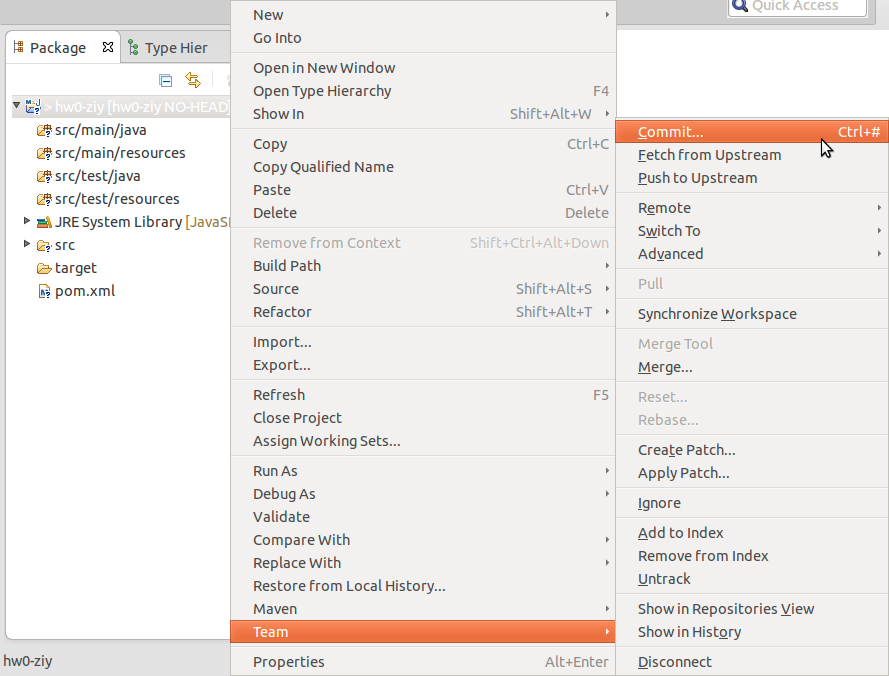
\includegraphics[scale=0.3]{project-19-git-commit}
\caption{Performing a git-commit\label{project-19-git-commit}}
\end{figure}

You should see a ``greater than'' symbol between the project icon and your
project name (see Figure \ref{project-19-git-commit}, which means you have made
some changes to the project so that there exist some differences between your
current workspace version and the branch head. Question marks on the project
element icon represent the corresponding elements are not indexed yet. You might
be wondering what changes you've made because you thought you haven't written
any code. Actually, you have created a Maven project, which process will
generate the \verb|pom.xml| file, and modified the Eclipse configuration files.
So let's perform our first git-commit.

\begin{enumerate}

\item Right-click on the project name, and select \textbf{Team} $\rightarrow$
\textbf{Commit\ldots}. See Figure \ref{project-19-git-commit}, and then type in
your username and email address on GitHub in the popup ``Identify Yourself''
message window.

\begin{figure}[t]
\centering
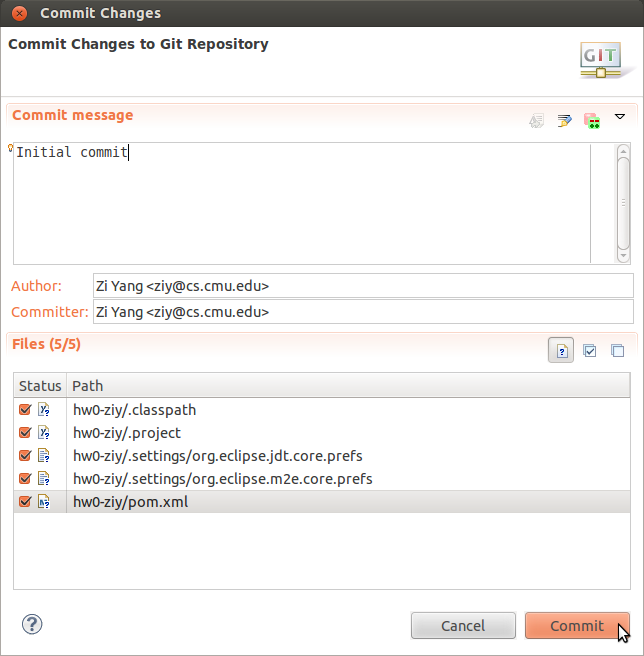
\includegraphics[scale=0.3]{project-21-git-commit-message}
\caption{Viewing and confirming commit message\label{project-21-git-commit-message}}
\end{figure}

\begin{figure}[t]
\centering
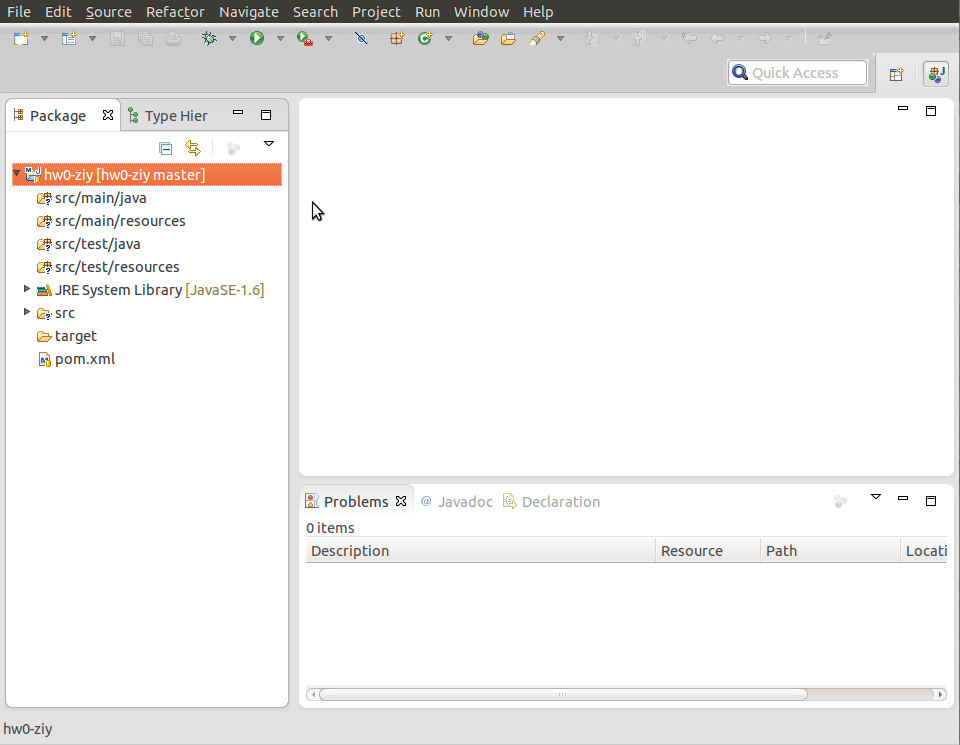
\includegraphics[scale=0.3]{project-22-git-commit-done}
\caption{Committed project\label{project-22-git-commit-done}}
\end{figure}

\item In the ``Commit Changes'' window, you are allowed to choose the files you
want to commit (and also automatically add to the index). As you can see in
Figure \ref{project-21-git-commit-message}, during creating the empty Maven
project, several Eclipse and Maven related configuration files are generated.
Moreover, type in a commit message to describe what changes you've made and
leave your name as well as your email address (which is a convention) in the
committer field. Finally, by clicking \textbf{Commit}, you've done with your
first git-commit. You can see in Figure \ref{project-22-git-commit-done}, the
``greater than'' symbol disappears, and the question marks on the committed
files become a repository icon, which means the files are in the latest version.
You could also find your git-commit helps the code merge into the new master
branch from a NO-HEAD branch.

If you are using SVN, then you've done with sychronizing your local workspace
with the remote repository once you execute a commit command, but remember the
feature of Git? Your project repository is distributed, which means your
previous git-commit conceptually affects all your project repositories, but in
fact you should make it happen with an additional \emph{push}. A nice picture at
\url{http://gitready.com/beginner/2009/01/21/pushing-and-pulling.html} may help
you better understand what is actually happening when you perform git commit,
add, push, fetch, pull, etc.

\begin{figure}[t]
\centering
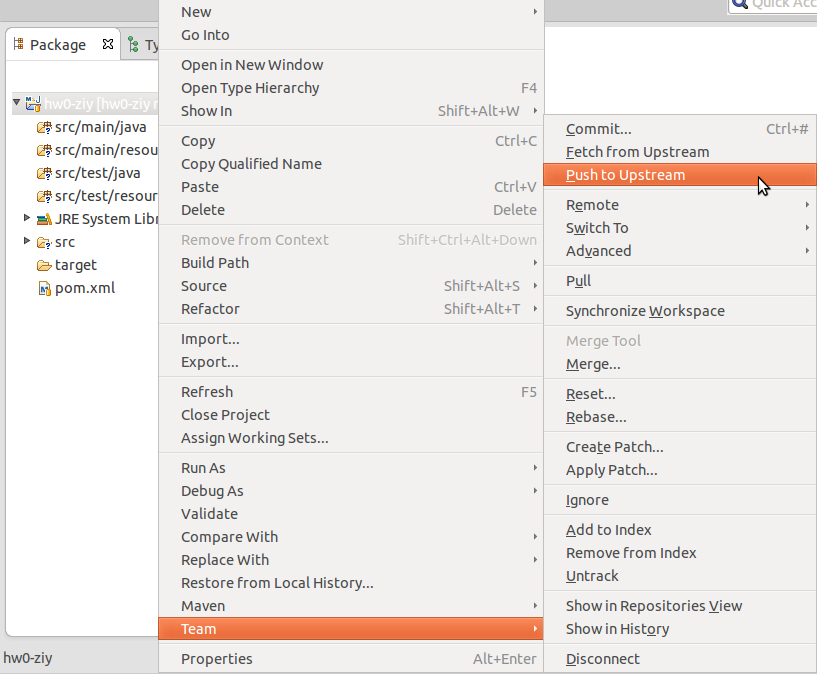
\includegraphics[scale=0.3]{project-23-git-push}
\caption{Performing a git push\label{project-23-git-push}}
\end{figure}

\item Right-click on the project name, and select \textbf{Team} $\rightarrow$
\textbf{Push to Upstream}. See Figure \ref{project-23-git-push}.

\begin{figure}[t]
\hspace{-2em}
\begin{minipage}{0.5\textwidth}
\centering
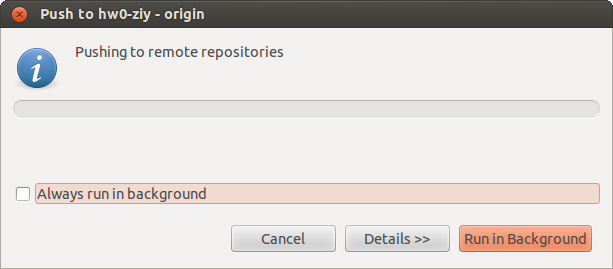
\includegraphics[scale=0.3]{project-24-git-push-progress}
\caption{Viewing the git push progress\label{project-24-git-push-progress}}
\end{minipage}
\hfill
\begin{minipage}{0.5\textwidth}
\centering
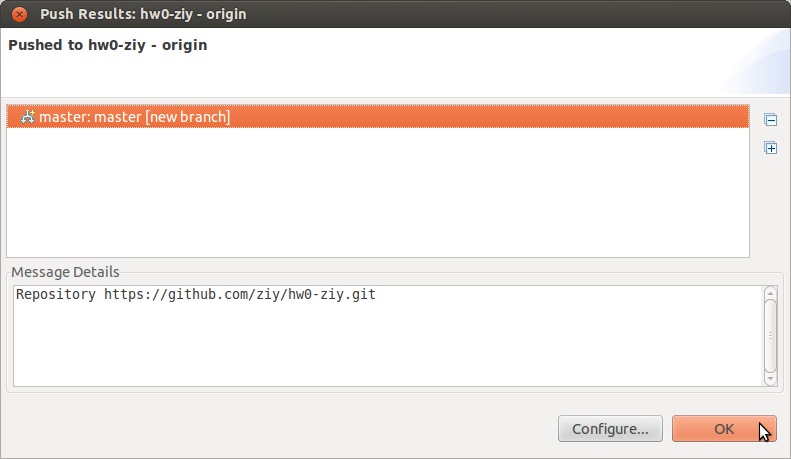
\includegraphics[scale=0.3]{project-25-git-push-result}
\caption{Viewing the git push result\label{project-25-git-push-result}}
\end{minipage}
\hspace{-1em}
\end{figure}

\item Now you can see a progress indication window pops up (see Figure
\ref{project-24-git-push-progress}), which says \textbf{Pushing to remote
repositories}.

\item Finally, you could see the push results in the ``Push Results'' window.
Click \textbf{OK} to close the window and get back to your workspace.

\end{enumerate}

In your next homework, you will need to use other Git commands within Eclipse.



\section{Creating Maven project from the archetype}

For this homework, we create another archetype called
\texttt{hellobioqa-archetype} to help you quickly get your development started.
We briefly show you the process you've gone through for your Homework 1.

\begin{enumerate}

\item Open your Eclipse's \textbf{Preferences} window, and navigate to
\textbf{Maven} $\rightarrow$ \textbf{Archetypes}, and click \textbf{Add Remote
Catalog\ldots}.

\item Type the following URL into the \textbf{Catalog File} field.

\small
\begin{verbatim}
http://ziy.github.com/hellobioqa-archetype/repository/archetype-catalog.xml
\end{verbatim}
\normalsize

Optionally, you can add a \textbf{Description} for this catalog, for example
``HelloBioQA Catalog''. Then click \textbf{OK} on the \textbf{Remote Archetype
Catalog} window and another \textbf{OK} on the \textbf{Preferences} window.

\item Include the following lines in your \texttt{settings.xml} in order to
download the artifact if you didn't do so in Homework 1.

\lstinputlisting[language=XML,float,linewidth=1.1\textwidth,caption=Configuring settings.xml,label=settings]{settings.xml}

\item Now you can follow almost the same steps to import to Eclipse as you did
for Homework 1. Since we have created the archetype for you, remember to
unselect \textbf{Create a simple project (skip archetype selction)}. Then click
\textbf{Next}.
 
\item Here you can select ``HelloBioQA Catalog'' (or other names you specified
in the previous step) or ``All Catalogs'' in the drop-down menu for
\textbf{Catalog}. Then, type in ``hellobioqa-archetype'' (without quotes) in the \textbf{Filter}
field, and in order to get the latest snapshot archetypes, you need to check
\textbf{Include snapshot archetypes} as well. Select the archetype listed below,
and click next to continue.

\item In the next window, you are asked to specify the \textbf{Group Id} and
\textbf{Artifact Id}. Similar to Homework 0 and 1, the Group Id is

\begin{center}
\textbf{edu.cmu.lti.11791.f13.hw2}
\end{center}

and Artifact Id is

\begin{center}
\textbf{hw2-teamXX}
\end{center}

with XX being your team number. Since we also included two sample components for
retrieval strategist and passage extraction within a particular, remember to
specify \texttt{Package} as

\begin{center}
\textbf{edu.cmu.lti.oaqa.openqa.hellobioqa}
\end{center}

See Figure \ref{fig:package-name}. Then click \textbf{Finish}.

\begin{figure}[t]
\centering
\includegraphics[scale=0.3]{package-name}
\caption{Parameters to create a Maven artifact from archetype\label{fig:package-name}}
\end{figure}

\item You need to edit the \texttt{pom.xml} file to type in the SCM information
of your GitHub repository for Homework 2 as you did in Homework 0.

\item You also need to manually edit the \texttt{launches/hellobioqa.launch}
file. Open the file, replace the \verb|${project_name}| with your project name
(e.g., \verb|hw2-team00|).

\item Probably you want to add another line into launch file to give extra
memory to run the pipeline, like the following

\begin{verbatim}
<stringAttribute key="org.eclipse.jdt.launching.VM_ARGUMENTS" value="-Xmx1g"/>
\end{verbatim}

\item Same as before, you probably need to right-click the project name, and
click \textbf{Maven} $\rightarrow$ \textbf{Update Project} to download the
dependencies.

\end{enumerate}

You can see that we have included

\begin{itemize}

\item the \texttt{pom.xml}. You can go to the \textbf{Dependencies} tab after
you double-click the pom file, and you will be able to see your project only
depends on \texttt{helloqa} project, which brings simple implementations for all
the phases described in \texttt{baseqa} project. You won't need any direct
dependency on any UIMA SDK package, which are essential to your Homework 1.

If you want to take a look at what are inside \texttt{helloqa} project and
other indirect dependencies, you can unfold the \texttt{Maven Dependencies}
folder under your project name in the Package Explorer View.

\item input file in the \texttt{src/main/resources/input} folder, and
gold-standard annotations in the \texttt{src/main/resources/gs} folder. If you
are interested in their contents, you can open them with a text editor.

\item several descriptors under \texttt{src/main/resources/hellobioqa} directory
and subdirectories. All of them are specific to the hellobioqa task, and
actually, you can find more descriptors from dependencies, e.g.,
\texttt{helloqa}, \texttt{jdbc-provider}, etc. These descriptors can also be
considered to incorporate in your project.

\item the main yaml \texttt{src/main/resources/hellobioqa/hellobioqa.yaml}

\item an Eclipse launch file \texttt{launches/hellobioqa.launch}. To run the
pipeline, you can right-click this file in the Package Explorer View, and then
click \textbf{Run As} $\rightarrow$ \textbf{hellobioqa}.

\item a local database version of the cse repository
\texttt{data/oaqa-eval.db3}. All your experiment intermediate result and
evaluation results will be permanently stored here (unless you manually delete
table entries), and you will find the file may grow to several megabytes after
thundreds of experiments. Therefore, we suggest you should not commit this file
to the GitHub repository, instead you can \texttt{git ignore} this file to avoid
this huge file bothering you every time you commit your project.

\end{itemize}

Before you commit and push all the initial code changes to GitHub repository, we
suggest you to first test if you can successfully run the pipeline.

\begin{enumerate}

\item Right-click this file in the Package Explorer View, and then click
\textbf{Run As} $\rightarrow$ \textbf{hellobioqa}. Wait until all 28 questions
are processed, and the evaluation results are printed to the console, and you
find no exceptions are thrown.

\item Git-ignore \texttt{data/oaqa-eval.db3}\footnote{Since your team member
also needs the database file to run experiment, the team leader can add it to
the index first then remove it after team members clone the project to their
machines, or all the members can download an empty file from here:
\url{https://github.com/oaqa/helloqa/blob/a051e1233be92bca309ff8761835fce412f6bfd5/data/oaqa-eval.db3?raw=true},
and put it under \texttt{data/}.}, and commit/push all other code changes to the
GitHub repository. Remember to commit the .project file, .classpath file and all
other important configuration files from your project root directory, and it
will be helpful for your team members to directly import an existing project.

\item Now, other team members are able to clone the repository to their
workspaces and start working on particular task. When you are asked to
\textbf{Select a wizard to use for importing projects}, don't forget to select
\textbf{Import existing projects} as long as your team leader commited .project
and .classth to the repository.

\end{enumerate}



\section{Eclipse (Git, Maven plug-ins integrated)}

If you have an Eclipse IDE for Java Developers with version $\ge$ 3.7, you could
probably skip this task. But if you are stuck in a situation where you were told
Eclipse is missing a plug-in, you might want to return to this section. If you
have other packages (Eclipse Classic or Eclipse for Java EE Developers), please
do not skip this task.

\begin{enumerate}

\item Download Eclipse IDE for Java Developers 4.3 at
\url{http://www.eclipse.org/downloads}.

\begin{qa}

\item[Q1] Can I use an older version of Eclipse?

\item[A1] You can try to use an older version, but some plug-ins (e.g., m2e)
might complain about the Eclipse version if it is older than 3.7.

\item[Q2] Can I use other Eclipse packages?

\item[A2] Eclipse IDE for Java Developers includes almost all the Eclipse
components (jdt, EGit, m2e, and so on) we need for this course. You could also
work with other packages, e.g., Eclipse IDE for Jave EE Developers or Eclipse
Classics, and as they don't come with such plugins by default, you have to
install these plug-ins all by yourself.

\end{qa}

\item Install Eclipse by simply uncompressing the downloaded package.

\begin{figure}[t]
\centering
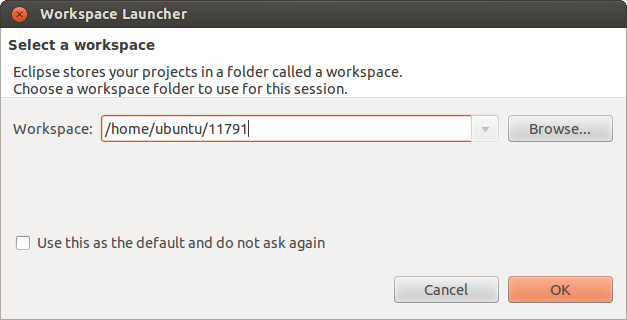
\includegraphics[scale=0.3]{eclipse-01-login}
\caption{Eclipse choose workspace\label{eclipse-01-login}}
\end{figure}

\item Use the default workspace path or create your own workspace, as shown in
Figure \ref{eclipse-01-login}. And finally, we could see the Eclipse Welcome
view at the end of workspace initialization. See Figure
\ref{eclipse-02-welcome}.

\begin{figure}[t]
\centering
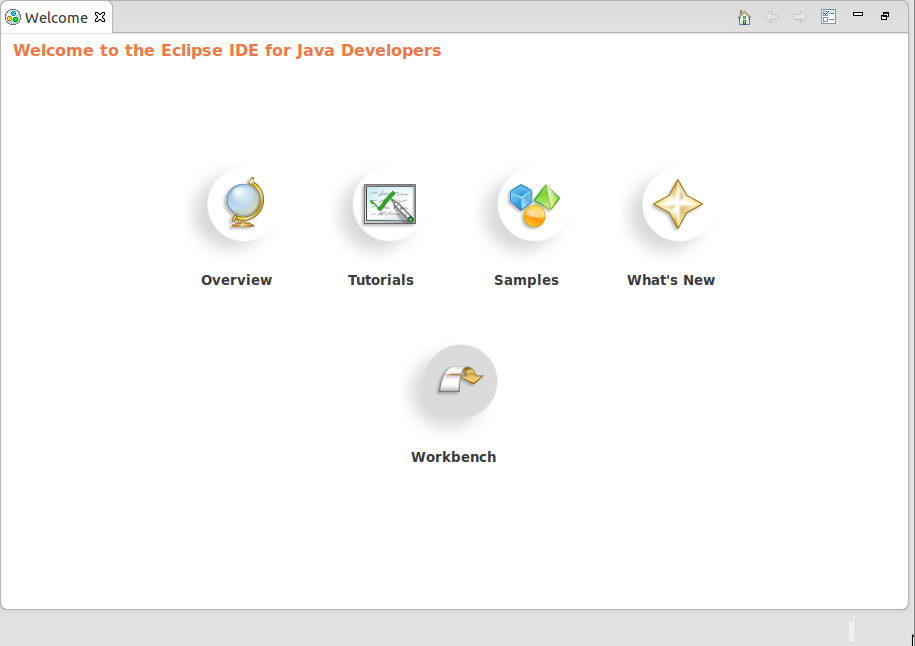
\includegraphics[scale=0.3]{eclipse-02-welcome}
\caption{Eclipse Welcome view\label{eclipse-02-welcome}}
\end{figure}

\end{enumerate}


That's the start of your developement. From now on, everthing will become less
platform specific, and we will show you how to configure the workspace, create
your Maven project and release it in the rest of the homework.


\section{A Little Configuration}

\subsection{Letting m2e know your password}

\begin{enumerate}

\item Click \textbf{Edit} (or \textbf{Window} depending on your OS)
$\rightarrow$ \textbf{Preferences}, and choose \textbf{Maven} $\rightarrow$
\textbf{User Settings}, and find the default Maven setting path for your system.
See Figure \ref{eclipse-03-maven-setting}.

\item Create the \verb|settings.xml| file at the given directory, and copy the
text in Listing \ref{settings} into the file, which will store your ID and
passwords. Remember to replace \verb|ID| and \verb|PASSWORD| with your personal
Maven project repository account we provide you, and also don't upload this file
to any remote repository or share it with others.

\item Go back to \textbf{Edit} (or \textbf{Window}) $\rightarrow$
\textbf{Preferences}, and choose \textbf{Maven} $\rightarrow$ \textbf{User
Settings} again, you will see the plugin could find the setting file you
specified (see Figure \ref{eclipse-04-maven-setting-back}).
% and click \textbf{Update settings}. You will be able to see the repository is
% now being refreshed.

\begin{figure}[t]
\hspace{-3em}
\begin{minipage}{0.5\textwidth}
\centering
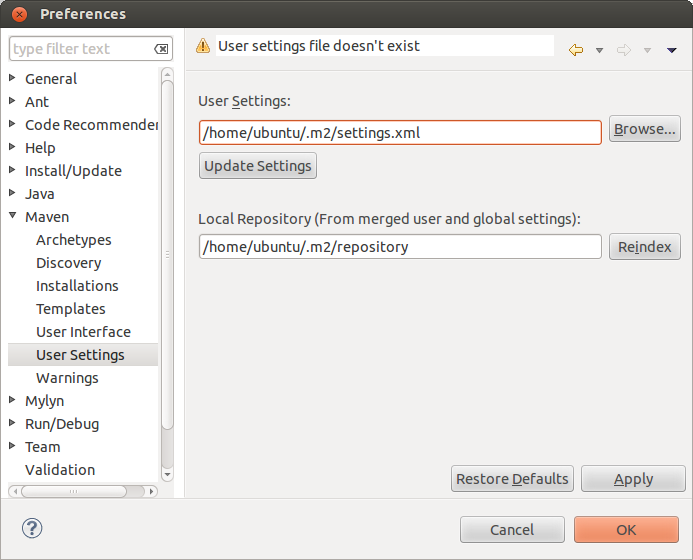
\includegraphics[scale=0.3]{eclipse-03-maven-setting}
\caption{Eclipse maven user profile setting\label{eclipse-03-maven-setting}}
\end{minipage}
\hfill
\begin{minipage}{0.5\textwidth}
\centering
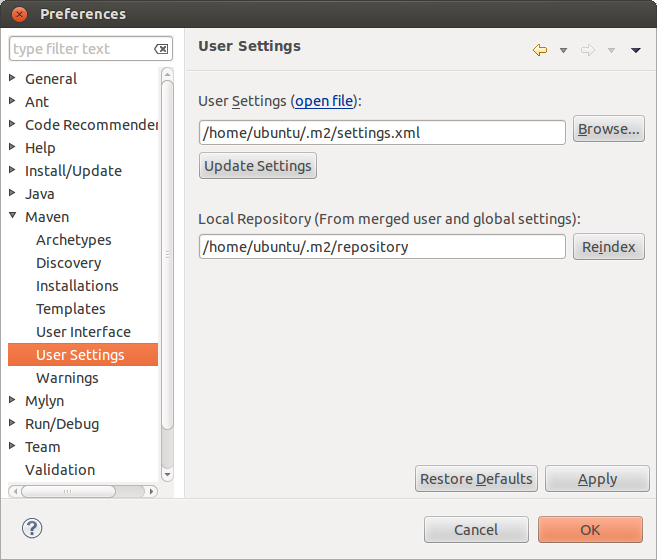
\includegraphics[scale=0.3]{eclipse-04-maven-setting-back}
\caption{Eclipse maven user profile setting\label{eclipse-04-maven-setting-back}}
\end{minipage}
\hspace{-3em}
\end{figure}

\lstinputlisting[language=XML,float,linewidth=1.1\textwidth,caption=Configuring settings.xml,label=settings]{settings.xml}

\end{enumerate}

\subsection{Importing Apache UIMA code style template}

To development a software as a team, members should always adopt the same code
conventions to improve the readability and maintainability of the project. We
suggest you to view the \emph{Code Conventions for the Java Programming
Language} at \url{http://www.oracle.com/technetwork/java/codeconv-138413.html},
which was published from Oracle. For our course homeworks, you are required to
adopt a set of more specific coding conventions from Apache UIMA project.
Details can be found at \url{http://uima.apache.org/codeConventions.html}. At
the bottom of the page, you could find a link to download the Eclipse code style
template\footnote{\url{http://uima.apache.org/downloads/ApacheUima_EclipseCodeStylePrefs.xml}}.

\begin{enumerate}
\item Download the template and save it in your local filesystem.
\item Click \textbf{Window} $\rightarrow$ \textbf{Preferences}, then go to \textbf{Java} $\rightarrow$ \textbf{Code Style} $\rightarrow$ \textbf{Formatter}, and click \textbf{Import\ldots}. 
\end{enumerate}

Remember before you finish editing a Java file, press \textbf{Ctrl+Shift+F} to
perform an automatic code formation.

Another optional but useful tool for you to check your code style is the Eclipse
Checkstyle plug-in. You can learn how to download and install the plug-in at
\url{http://eclipse-cs.sourceforge.net/}.

